\subsection{Tree Methods}
\label{sec:methods.structured.tree}

% Author: Flo

With Tree Methods, features are assumed to have a certain structure, where
features can be grouped into groups, and these groups can again be grouped into
groups, until there is only one group left.

This index-tree-structure can be visualized as tree, with all features being
leafes (see Figure \ref{fig:methods.structured.tree.lasso}).

\begin{figure}[!ht]
  \centering 
  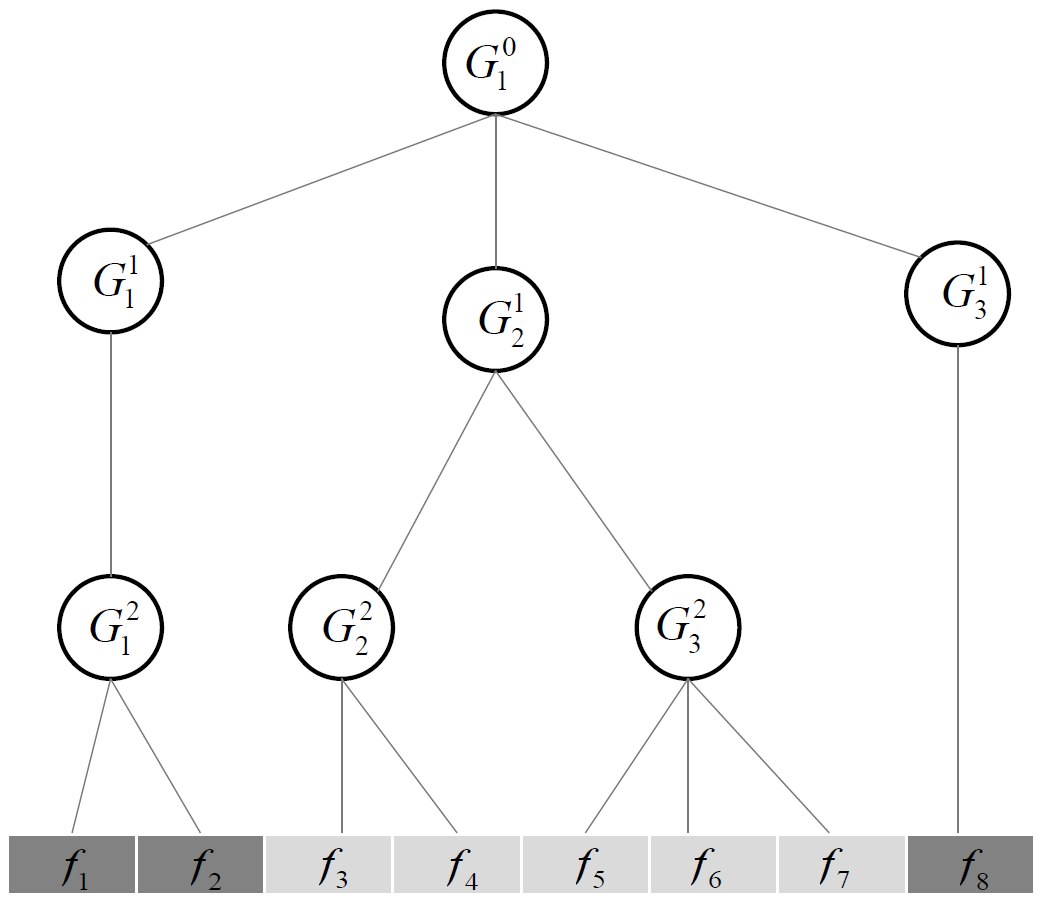
\includegraphics[width=0.5\textwidth]{chapters/methods/structured/tree_lasso}
  \caption{Reprinted from (\cite{Tang:04}). Illustration of an index tree.
  E.g. Features $f_1$ and $f_2$ can be grouped into $G_1^2$ (\cite{Tang:04}).}
  \label{fig:methods.structured.tree.lasso}
\end{figure}

Using index-trees, methods like the tree structured group Lasso (\cite{Kim:10})
can use this structure to eliminate tree-nodes on a higher level of the hierachy and
therefore eliminate many features at once.